\documentclass{article}%
\usepackage[T1]{fontenc}%
\usepackage[utf8]{inputenc}%
\usepackage{lmodern}%
\usepackage{textcomp}%
\usepackage{lastpage}%
\usepackage[head=40pt,margin=0.5in,bottom=0.6in]{geometry}%
\usepackage{graphicx}%
%
\title{\textbf{Denuncian que escasez de antirretrovirales en Venezuela es de 95\%}}%
\author{EFE}%
\date{01/12/2018}%
%
\begin{document}%
\normalsize%
\maketitle%
\textbf{URL: }%
http://www.el{-}nacional.com/noticias/crisis{-}humanitaria/denuncian{-}que{-}escasez{-}antirretrovirales{-}venezuela\_261799\newline%
%
\textbf{Periodico: }%
EN, %
ID: %
261799, %
Seccion: %
Crisis humanitaria\newline%
%
\textbf{Palabras Claves: }%
Salud, Crisis humanitaria\newline%
%
\textbf{Derecho: }%
2.1, %
Otros Derechos: %
, %
Sub Derechos: %
2.1.1\newline%
%
\textbf{EP: }%
NO\newline%
\newline%
%
\textbf{\textit{La ONG Acción Ciudadana Contra el Sida pidió a los gobiernos del mundo ayuda humanitaria para detener la muerte de miles de personas por falta de medicinas y alimentos~}}%
\newline%
\newline%
%
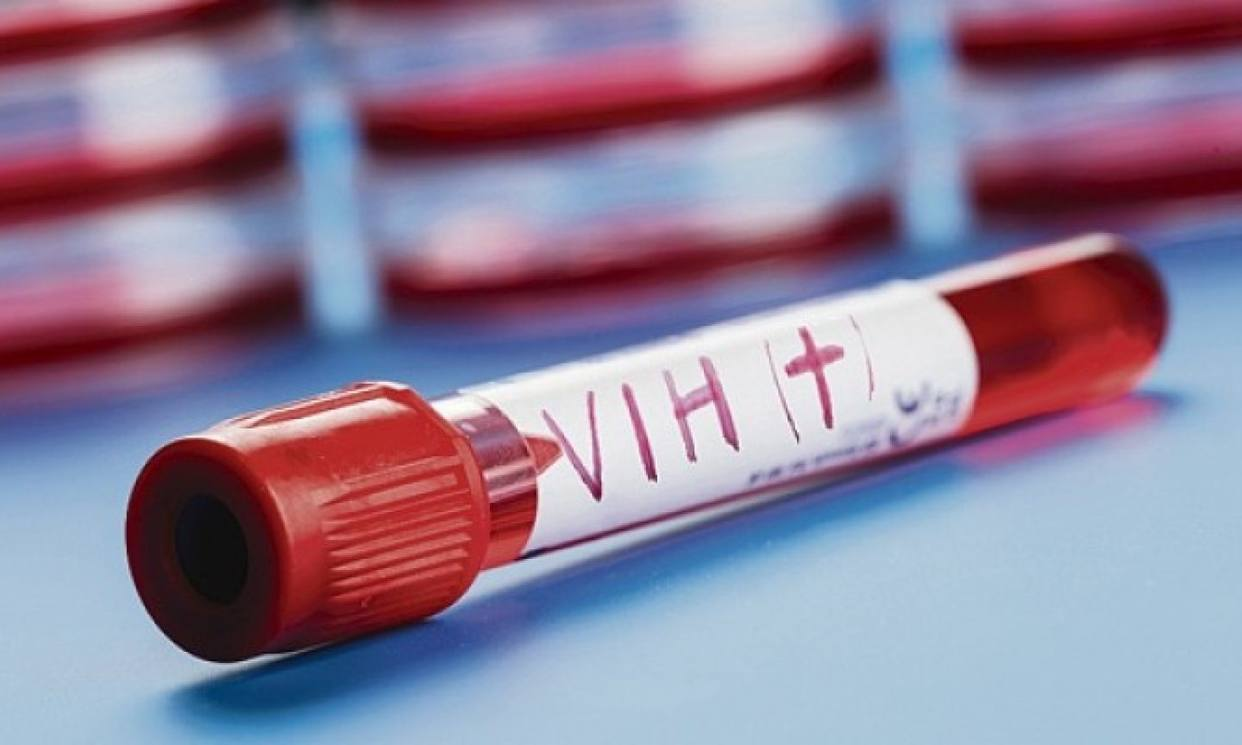
\includegraphics[width=300px]{24.jpg}%
\newline%
%
La ONG Acción Ciudadana Contra el Sida denunció este sábado en el Día Mundial de la Lucha contra el Sida que en~Venezuela~hay una escasez de 95\% de medicamentos antirretrovirales y pidió ayuda humanitaria, en medio de la severa crisis económica que atraviesa el país.%
\newline%
%
"Hoy \#Diamundialcontraelsida en \#Venezuela existe más de 95\% de desabastecimiento de medicamentos antirretrovirales porque el gobierno no los compra desde el año 2017. Miles de personas con VIH mueren por esta causa. La maldad y la incapacidad rige la salud pública venezolana", dijo en Twitter la ONG.%
\newline%
%
La organización, que realizará, junto a la Red Venezolana de Gente Positiva, el próximo martes un foro sobre el VIH en el contexto de la "crisis humanitaria" que vive el país, agregó en otro mensaje que los hospitales del país se encuentran "sin reactivos para diagnosticar" la enfermedad y su carga viral.%
\newline%
%
Denunció también que a las embarazadas con VIH les niegan atención médica en centros públicos de salud en el momento del parto.%
\newline%
%
Pidió a todos los gobiernos del mundo ayuda humanitaria para detener las miles de muertes de personas por falta de antirretrovirales y alimentos.%
\newline%
%
La ONG Acción Solidaria también manifestó que las personas con VIH en~Venezuela~no están recibiendo su tratamiento antirretroviral con regularidad.%
\newline%
%
Esta misma ONG denunció la semana pasada en una entrevista al portal~Caraota Digital~que estiman que 10.000 de las 70.000 personas que registran con VIH han emigrado en busca de tratamiento.%
\newline%
%
Sin embargo, no hay certezas de los datos en los últimos dos años de las personas que viven con este virus en el país, según dijo a Efe en septiembre pasado la representante ONU{-}SIDA en~Venezuela, Regina López.%
\newline%
%
En aquella oportunidad, López señaló la imposibilidad de hacer diagnósticos en algunos hospitales y la escasez de antirretrovirales como dos problemas en~Venezuela~que, consideró, "no le ha sido fácil" de resolver al gobierno. "Sobre todo después de estas restricciones de dinero", dijo, en alusión a las sanciones económicas que le impusieron este año.%
\newline%
%
Como parte de la lucha contra el sida en~Venezuela, la Defensoría del Pueblo, en conjunto con ONU{-}SIDA, el Fondo de las Naciones Unidas para la Infancia (Unicef) y otros entes del Estado venezolano, inició este viernes en Caracas una campaña para informar sobre el derecho a la igualdad y la no discriminación.%
\newline%
%
La campaña, que se extenderá hasta la próxima semana,~tiene el lema "No a la Discriminación de Personas con VIH".%
\newline%
%
\end{document}